% This is "sig-alternate.tex" V2.0 May 2012
% This file should be compiled with V2.5 of "sig-alternate.cls" May 2012
%
% This example file demonstrates the use of the 'sig-alternate.cls'
% V2.5 LaTeX2e document class file. It is for those submitting
% articles to ACM Conference Proceedings WHO DO NOT WISH TO
% STRICTLY ADHERE TO THE SIGS (PUBS-BOARD-ENDORSED) STYLE.
% The 'sig-alternate.cls' file will produce a similar-looking,
% albeit, 'tighter' paper resulting in, invariably, fewer pages.
%
% ----------------------------------------------------------------------------------------------------------------
% This .tex file (and associated .cls V2.5) produces:
%       1) The Permission Statement
%       2) The Conference (location) Info information
%       3) The Copyright Line with ACM data
%       4) NO page numbers
%
% as against the acm_proc_article-sp.cls file which
% DOES NOT produce 1) thru' 3) above.
%
% Using 'sig-alternate.cls' you have control, however, from within
% the source .tex file, over both the CopyrightYear
% (defaulted to 200X) and the ACM Copyright Data
% (defaulted to X-XXXXX-XX-X/XX/XX).
% e.g.
% \CopyrightYear{2007} will cause 2007 to appear in the copyright line.
% \crdata{0-12345-67-8/90/12} will cause 0-12345-67-8/90/12 to appear in the copyright line.
%
% ---------------------------------------------------------------------------------------------------------------
% This .tex source is an example which *does* use
% the .bib file (from which the .bbl file % is produced).
% REMEMBER HOWEVER: After having produced the .bbl file,
% and prior to final submission, you *NEED* to 'insert'
% your .bbl file into your source .tex file so as to provide
% ONE 'self-contained' source file.
%
% ================= IF YOU HAVE QUESTIONS =======================
% Questions regarding the SIGS styles, SIGS policies and
% procedures, Conferences etc. should be sent to
% Adrienne Griscti (griscti@acm.org)
%
% Technical questions _only_ to
% Gerald Murray (murray@hq.acm.org)
% ===============================================================
%
% For tracking purposes - this is V2.0 - May 2012

\documentclass{sig-alternate}
\usepackage{graphicx}
\usepackage{caption}
\usepackage{subcaption}
\usepackage[utf8]{inputenc}
\usepackage{units}
\usepackage{url}
\usepackage{nicefrac}
\newcommand{\rpm}{\raisebox{.2ex}{$\scriptstyle\pm$}}

\begin{document}
%
% --- Author Metadata here ---
\conferenceinfo{WOODSTOCK}{'97 El Paso, Texas USA}
%\CopyrightYear{2007} % Allows default copyright year (20XX) to be over-ridden - IF NEED BE.
%\crdata{0-12345-67-8/90/01}  % Allows default copyright data (0-89791-88-6/97/05) to be over-ridden - IF NEED BE.
% --- End of Author Metadata ---

\title{Real Time Stereo Source Separation Plugin\titlenote{(Produces the permission block, and
copyright information). For use with
SIG-ALTERNATE.CLS. Supported by ACM.}}


\numberofauthors{2} %  in this sample file, there are a *total*
% of EIGHT authors. SIX appear on the 'first-page' (for formatting
% reasons) and the remaining two appear in the \additionalauthors section.
%
\author{
% You can go ahead and credit any number of authors here,
% e.g. one 'row of three' or two rows (consisting of one row of three
% and a second row of one, two or three).
%
% The command \alignauthor (no curly braces needed) should
% precede each author name, affiliation/snail-mail address and
% e-mail address. Additionally, tag each line of
% affiliation/address with \affaddr, and tag the
% e-mail address with \email.
%
% 1st. author
\alignauthor
Xinyuan Lai\\
       \affaddr{Center for Music Technology}\\
       \affaddr{Georgia Institute of Technology}\\
       \email{laixinyuan@gatech.edu}
\alignauthor
Yuxi Zhang\\
       \affaddr{Center for Music Technology}\\
       \affaddr{Georgia Institute of Technology}\\
       \email{yzhang453@gatech.edu}
}


\maketitle

\begin{abstract}

In this paper we present a real time audio plugin for stereo source separation, utilizing the spatial information hidden in the stereo audio signal. An improvement has been made upon the existing source separation algorithm. A graphical interface is presented for the user to specify the azimuth and opening angle for passing or rejecting the sound source from that spatial location. Three modes and filter types are provided to expand the usage of the plugin.  The testing and evaluation results are presented to demonstrate the usability and stability of the system. 

\smallskip

\end{abstract}


% A category with the (minimum) three required fields
\category{H.5.5}{Information Interfaces and Presentation}{Sound and Music Computing}[Signal analysis, synthesis, and processing]
%A category including the fourth, optional field follows...
%\category{D.2.8}{Software Engineering}{Metrics}[complexity measures, performance measures]

\terms{Algorithms}

\keywords{Stereo Souce Separation, Audio Plugin}

\section{Introduction}

The field of stereo source separation has seen many algorithms and designs based on time-frequency masks for different application tasks (compare \cite{Nakadai:02, Araki:09, Cobos:08, Woodruff:06, Vincent:06}).  The campaign of stereo audio source separation\footnote{\url{http://www.irisa.fr/metiss/SASSEC07/?show=intro}} provides valuable data sources for source separation algorithm tests and evaluation \cite{Vincent:07, Vincent:12}. 

    Our system comes as an audio plugin that works in real time for stereo input, utilizing the spatial information hidden in the stereo signal to accomplish source separation. The user can manually specify the azimuth and opening angle to pass or reject the sound source from that spatial location. Three different modes and filter types are available for adjusting to different use cases. In this paper, we are more focused on the design and implementation of the plugin, as well as several addon functionalities from the audio software engineering point of view. 

    The paper is organized as follows. Section~\ref{sec:algorithm_desc} briefly describes the algorithm used in our system, including the basic and improved algorithm design. Section~\ref{sec:implementation} describes the plugin implementation in detail, including the framework, class structure and third party library. Section~\ref{sec:GUI} displays the graphical interface design. The following Sect.~\ref{sec:evaluation} presents the results and existing problems. Section~\ref{sec:conclusion} concludes the paper. 

\section{Algorithm}\label{sec:algorithm_desc}

\subsection{Baisic Algorithm}

Our source separation plugin is based on an algorithm called \textsl{Azimuth Discrimination and Resynthesis} (ADRess) \cite{Barry:04, Barry2:04}, which is a time-frequency processing algorithm utilizing the difference between left and right channels' spectrograms resulting from the panning to filter out the specific source. So in real-time application, a phase-vocoder block-by-block structure, as well as implantation of input and output buffer is needed, in addition to the implementing the algorithm itself.
   
The basic idea of this algorithm is to tune down the magnitude of one of the stereo channels by ratios in equal intervals to find time-frequency points from left and right channels that cancel each other, regarding the cancelation point in the same tuning-down ratio from the same spatial source. The tuning-down ratio is called \textsl{azimuth} in this context. After turning the cancellation points into spectral peaks, the peaks from the same azimuth can be resynthesized to construct the signal from one spatial source. 

To reduce artifacts, the algorithm allows resynthesizing peaks from a range of azimuths, so that users can trade between separation effect and artifacts for their own preferences. 

Basically, there are two main controlling parameters for the algorithm: the azimuth and the opening angle for sound collection, which are integrated in our plugin as the two main control freedoms.


\subsection{Improved Design}

During the algorithm research and implementation, we found some minor bugs and restrictions in the original paper, so we fixed bugs and extend the algorithm to get better sound.
    
In the original paper, when resynthesizing the source from the center, what is really resynthesized is the center source AND all the components that exist exclusively in the selected channel. We fixed this bug by expanding the azimuth range.

To get a better sound from the center, we apply two source separation processes instead of one, and put them respectively in the left and right channel output. So the user can have stereo output when resynthesizing the sound from the center.

The details of rejecting sources is not included in this paper. The intuitive way to implement it is to do the source separation the other way round, by just summing up all the magnitude peaks beyond the specified range. But one problem is that the source from the other channel cannot be included. We found out that the reason of the other channel being completely blocked is the calculation in converting cancelation point to magnitude peaks. We modified the calculation so that the signal from the other channel can be let in.

In addition to the algorithmic modification above, we added smoothing along the azimuth for each block to reduce artifacts. A frequency mask is also added to pass or reject specific frequency components in the signal.


\section{Implementation}\label{sec:implementation}

\subsection{Framework}
        
One of the easiest ways to build up an audio plugin framework is to use Juce\footnote{\url{http://www.juce.com/about-juce}}, which wraps up the APIs of different plugin formats, providing developers with a generic interface for plugin development across different platforms. Some small functions such as post-script that automatically places plugins into the plugin folder also saves the developers from tedious work of moving files.

\subsection{Class Structure}

The class structure of the project is straightforward. The two classes \textsl{PluginEditor} and \textsl{PluginProcessor} made by jucer\footnote{\url{http://www.juce.com/forums/introjucer/jucer}} are respectively responsive for the interface and audio processing. All algorithm-related parts are concealed into the \textsl{ADRess} class, which takes in blocks of audio samples, does the source separation processing and saves the output back to the original buffer.

\subsubsection{ADRess}

\textsl{ADRess} class is the core algorithmic part of the project. The interface of this class only includes get and set parameters and process data.

The class is initialized with two arguments: the block size and a beta value that is the azimuth resolution. Once initialized, these two values cannot be altered.
     
There are three parameters in this class. The first parameter is the plugin \textsl{mode}, determining whether it bypasses the signal, extracts the specified source or suppresses the source. The second parameter is the \textsl{azimuth} from which the user would like to hear the sound. The third parameter is \textsl{width}, the opening angle for sound collection. 
 
The data process interface is the \textsl{process} function. To address the restriction that this algorithm only works for stereo signal, the two input arguments are set to be \textsl{left} and \textsl{right} signal buffer separately. After processing, the data will be saved back to the input buffer.

\subsubsection{PluginProcessor}

The \textsl{PluginProcessor} class defines the data behavior of the plugin. It initializes buffer, sets and gets the parameters and processes the input signal. 
     
\textsl{processBlock} is the function that takes in blocks of data from the host and processes them. As the core algorithm is concealed in \textsl{ADRess} class that takes in data of FFT block size, the role of \textsl{processBlock} in {PluginProcessor} is to send to \textsl{ADRess} class blocks of data with a specified hop size.
     
An input and an output buffer are implemented in place within the \textsl{processBlock} function. They are sample-by-sample circular buffer, that checks at each sample whether there has been enough input samples to send \textsl{ADRess} an FFT block to process. After processed by \textsl{ADRess}, the data will be overlap-and-add in the output buffer. The proper setting of the initial value of \textsl{outputBufferWritePosition\_} ensures the minimum delay of the output.

The block size and hop size is currently immutable in the project. The preset block size and hop size is necessary for the quality of source separation, which is tested in algorithm prototyping with Matlab. The computational power of most ordinary computers is able to endure release build with the current block size and hop size. Table~\ref{tab:para} shows details of system parameters.

        \begin{table}
            \centering
            \caption{System parameters}
            \label{tab:para}
            \begin{tabular}{ c | c }
                \hline
                FFT size & 4096 \\
                Block size & 4096 \\ 
                Hop size & 1024 \\ 
                Overlap & 75\% \\ 
                Input buffer length & 4096 \\ 
                Output buffer length & 8192 \\ 
                \hline
              \end{tabular}
        \end{table}

\subsubsection{PluginEditor}

The \textsl{PluginEditor} class defines the graphical interface of the plugin. It uses Juce’s basic components:  ToggleButton, Slider, TextLabel and Button. The functionalities of these buttons, slider, and arrow are controlled by the button listener, slider listener, and mouse listener. Whenever an event is detected (mouse dragged, slider value changed, button clicked, etc.), the \textsl{setParameter} function in \textsl{PluginProcessor} gets called and new parameters are passed to the processor. 

The two sections of toggle buttons are correlated with each other. For instance, when “Bypass” mode is selected, all filter type toggles are automatically disabled. When the user switch to “Solo” or "Mute" mode, the filter type toggles become effective again. The user can also decide the cutoff frequency of low pass or high pass filtering by tuning the \textsl{Cutoff Frequency} slider. 


\subsection{Third Party Library}

\textsl{Kiss\_fft}\footnote{\url{http://sourceforge.net/projects/kissfft/}}, a third-party library, is used for FFT calculation in this project. It is in place, working only after including the source files. With an estimated speed around 30\% slower than FFTW, Kiss\_fft is sufficient to carry on the real-time processing work. Another good character of this library is its variable type. It uses \textsl{std::complex} for ordinary FFT, and there is a choice of \textsl{float-std::complex} for real number FFT. The float number for real number input is easy to read and write, and the \textsl{std::complex} enables the usage of complex calculation such as \textsl{plus}, \textsl{multiplication}, \textsl{std::abs}, \textsl{std::arg} and \textsl{std::polar}, which makes computation really easy.


\section{Graphic User Interface}\label{sec:GUI}

Our design goal is to keep the UI as simple and neat as possible, while maximizing its functionalities in an intuitive way. 

On the left side is a semi-circle that represents the sound area in front of the listener, assuming that the listener is standing at the center of the semi-circle. The arrow that representing the azimuth can be dragged to change the source direction, while the slider below the semi-circle is used for changing the open angle of the effective region. The direction (Left or Right), the exact azimuth angle and the open angle values are displayed above the semi-circle. Button “C” is used for directly going back to the center direction without changing the current width.

On the right side are functionality sections. The user can select whether he/she wants to \textsl{bypass} the system, \textsl{solo} it or \textsl{mute} it by toggling the corresponding buttons in the “Mode” section. The “Filter Type” section is for adding “no”, “low pass” or “high pass” filter on the effective region. The user can manually set the cutoff frequency by tuning the slider at the bottom. It ranges from 0 Hz to 8000 Hz. 

To differentiate different modes and filter types, we paint the effective area in the color corresponding to the buttons, making it more intuitive for the user to use, see examples in Fig.~\ref{fig:UI}. For instances, the top left image shows that the plugin is in “solo” mode with a “low pass” filter added on. The cutoff frequency is about $490$ {Hz}. The top right example shows that the plugin is in “bypass” mode. All the filter type toggles are disabled at this moment.

\begin{figure}
  \begin{minipage}{0.49\textwidth}
    \centering
    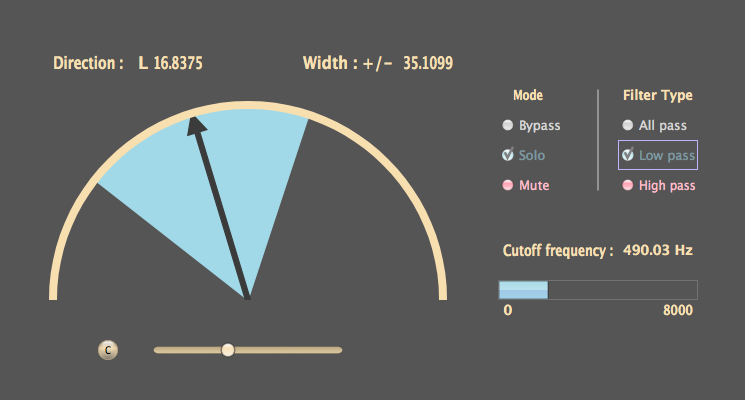
\includegraphics[width=.48\textwidth]{UI1}\quad
    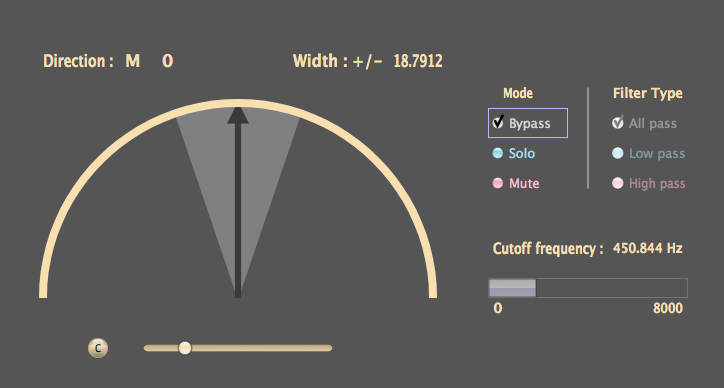
\includegraphics[width=.48\textwidth]{UI2}\\
    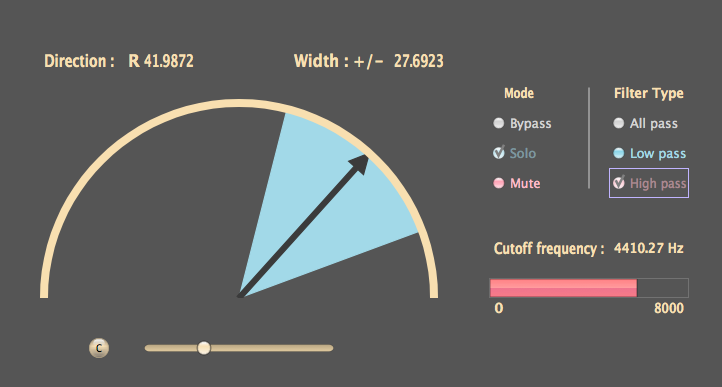
\includegraphics[width=.48\textwidth]{UI3}\quad
    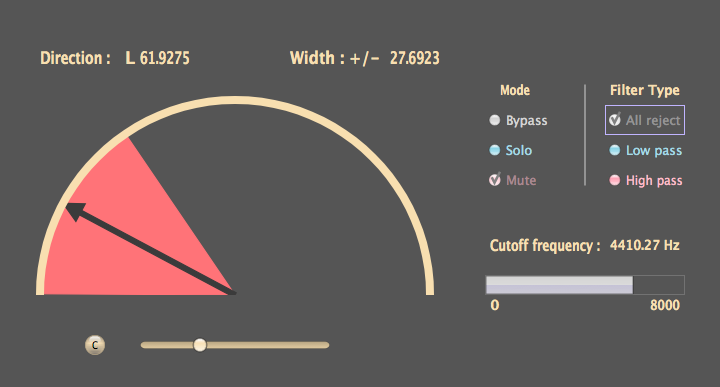
\includegraphics[width=.48\textwidth]{UI4}
    \caption{Plugin GUI with different modes}
    \label{fig:UI}
  \end{minipage}\\[1em]
\end{figure}
	

\section{Evaluation}\label{sec:evaluation}

Although there are objective evaluations for source separation algorithms, they are abstract to some degree and not necessarily useful in this context of plugin development. We mainly look into the subjective sound quality and stability of the plugin for the evaluation of the project. 
    
The plugin has a 4096 block size and 3/4 overlapping rate, high enough for a reasonable sound quality after phase-vocoder processing. The signal is added by Hann window and scaled down by a factor of 2 when bypassing, or is added a Hanning resynthesized and added window again when conducting source separation, ensuring no distortion with bypassing few clips with resynthesized signal. 

One existing issue is the typical phase-vocoder artifacts in the output, like the flickering grains of sound from isolate peaks in the spectrogram, or the bathroom-like artifacts. But by increasing the opening angle, the artifacts can be significantly reduced, bringing a much more natural sound.
     
With repeated tests, the plugin reflects good stability, and responds to user's operations fairly quickly. When dragging the arrow and slides on the GUI, the components and parameters are reacting responsively. Thanks to the sensitive parameter change and the nature of ADRess itself, fewer clicks are needed for changing the parameters.


\section{Conclusion}\label{sec:conclusion}

In this paper a stereo audio source separation plugin developed in C++ is presented. Based on the \textsl{Azimuth Discrimination and Resynthesis} algorithm, we implemented the basic methods as well as some improvements upon the existing algorithm. The user can specify the azimuth and opening angle for passing or rejecting the sound source from that spatial location. Several addon functionalities such as plugin mode, filter types and customized cutoff frequency are included in the system as well to expand the plugin usability. The system design, structure, implementation and testing results are discussed in details. A graphical interface is provided for the user to play with the plugin. Feedbacks with regards to the UI design and functionalities are very welcome.

For future work, more tests and evaluations with various types of sound is needed to verify the reliability of the plugin. We will also explore more ways to reduce the artifacts. Building a more systematic and complete source separation plugin based on what we have right now can be a good extension of this project.


\section{Acknowledgement}\label{sec:acknowledgement}
Our thanks to Prof. Lerch for all the guidance and valuable advises on this project.

\begin{thebibliography}{citations}

\bibitem {Nakadai:02}
Nakadai, Kazuhiro, Hiroshi G. Okuno, and Hiroaki Kitano:
``Real-time sound source localization and separation for robot audition,''
{\it INTERSPEECH},
2002.

\bibitem {Araki:09}
Araki, Shoko, et al.:
``Stereo source separation and source counting with MAP estimation with Dirichlet prior considering spatial aliasing problem,''
{\it Independent Component Analysis and Signal Separation},
Springer Berlin Heidelberg, 2009. 742-750.

\bibitem {Cobos:08}
Cobos, Maximo, and José J. López:
``Stereo audio source separation based on time–frequency masking and multilevel thresholding,''
{\it Digital Signal Processing},
18.6 (2008): 960-976.

\bibitem {Woodruff:06}
Woodruff, John F., Bryan Pardo, and Roger B. Dannenberg:
``Remixing Stereo Music with Score-Informed Source Separation,''
{\it ISMIR},
2006.

\bibitem {Vincent:06}
Vincent, Emmanue:
``Musical source separation using time-frequency source priors,''
{\it Audio, Speech, and Language Processing, IEEE Transactions on 14.1},
(2006): 91-98.

\bibitem {Vincent:07}
E. Vincent, H. Sawada, P. Bofill, S. Makino and J.P. Rosca:
``First stereo audio source separation evaluation campaign: data, algorithms and results,''
{\it in Proc. Int. Conf. on Independent Component Analysis and Signal Separation},
pp. 552-559, 2007.

\bibitem {Vincent:12}
E. Vincent, S. Araki, F.J. Theis, G. Nolte, P. Bofill, H. Sawada, A. Ozerov, B.V. Gowreesunker, D. Lutter and N.Q.K. Duong.:
``The Signal Separation Evaluation Campaign (2007-2010): Achievements and remaining challenges,''
{\it Signal Processing},
92, pp. 1928-1936, 2012.

\bibitem {Barry:04}
Barry, Dan, Bob Lawlor, and Eugene Coyle.:
``Sound source separation: Azimuth discriminiation and resynthesis,''
{\it},
2004.

\bibitem {Barry2:04}
Barry, Dan, Eugene Coyle, and Bob Lawlor.:
``Real-time sound source separation: Azimuth discrimination and resynthesis,''
{\it Audio Engineering Society Convention 117},
Audio Engineering Society, 2004.


\end{thebibliography}


\end{document}
